Para la validación del prototipo, se ha realizado una experiencia con el juego en veinte alumnos de un centro escolar de Murcia de 1º de la ESO. Se visitó el centro y se probó el juego durante dos horas en un aula, durante una sesión de clase, con la supervisión del profesor del aula.

\section{Encuestas}

De cara a validar el prototipo, la primera fuente de datos planteada fue preparar una encuesta (Disponible en el Anexo \ref{sec:apendice}) con la que obtener sensaciones e impresiones de primera mano de los alumnos.

El objetivo de estas preguntas es tanto obtener una idea general de si el prototipo verdaderamente está sirviendo como ayuda para desarrollar el PC, como comprobar si está sirviendo para divulgar acerca de la restauración de cosistemas, y además comprobar cómo de divertido y usable es como videojuego.

El resultado ha sido muy útil e ilustrativo, dado que el feedback ha sido increíblemente positivo. 

\section{Datos Cualitativos}

Por desgracia los datos recabados son ligeramente dispares y no representan la muestra total de alumnos que evaluamos con el juego (~20 alumnos), ya que el instituto tenía una serie de Firewalls que bloquearon las conexiones del prototipo con la BBDD.

Los datos recabados finalmente son:

\begin{compactitem}
    \item User\textunderscore Id - El id inequívoco de un usuario.
    \item Name - El usuario que hayan elegido.
    \item Gender - El Icono que hayan elegido.
    \item Age - La edad del usuario.
    \item Progress - La cantidad media de progreso de todas las fases (máximo 100).
    \item Machines Placed - La cantidad de máquinas colocadas.
    \item Machines Sold - La cantidad de máquianas vendidas.
    \item Success Phase - La cantidad de fases completadas.
    \item Failure Phase - La cantidad de fases reiniciadas.
    \item Duration - El tiempo de juego.
\end{compactitem}

\section{Experiencia de Validación}

La experiencia de la validación fue en general muy positiva, se pudo observar a los niños interactuar en tiempo real con el juego y ver dónde
 les costaba avanzar. El resultado es una vez más muy positivo dado que todos los alumnos menos cuatro fueron capaces de completar la demo.
  No obstante, la gran mayoría se atascó en la fase de relacionar problemas con otros problemas y consecuencias, por lo que quizás ese apartado
   no está bien explicado o es demasiado complejo para niños de esas edades.

Por otra parte, el ambiente en la clase fue muy bueno y la experiencia fue positiva y amena para todos los implicados, los profesores estuvieron 
de acuerdo en que utilizar este tipo de herramientas de forma didáctica es una muy buena forma de mejorar el ambiente en el aula sin dejar de enseñar
 a los alumnos. 

\section{Resultados Cuantitativos}

En primer lugar, podemos ver que en la representación de género (Figura \ref{fig:questionario_2}) ha habido bastante
 paridad (58 - 42\%). Además de poder encontrar que la distribución de regularidad a la hora de jugara videojuegos también 
 es bastante equitativa (Figura \ref{fig:questionario_3}) donde se puede observar que más o menos la mitad de los alumnos 
 jugaban a diario, y el resto se dividían entre semanalmente y casi nunca.

En base a los resultados obtenidos se puede comprobar también que la edad de los alumnos pudo haber sido un factor importante dado que cerca del 80\% de los alumnos de trece años completó la demo, mientras que solamente en torno al 60\% de alumnos de doce años lo logró.   

 \begin{figure}[H]
    \centering
      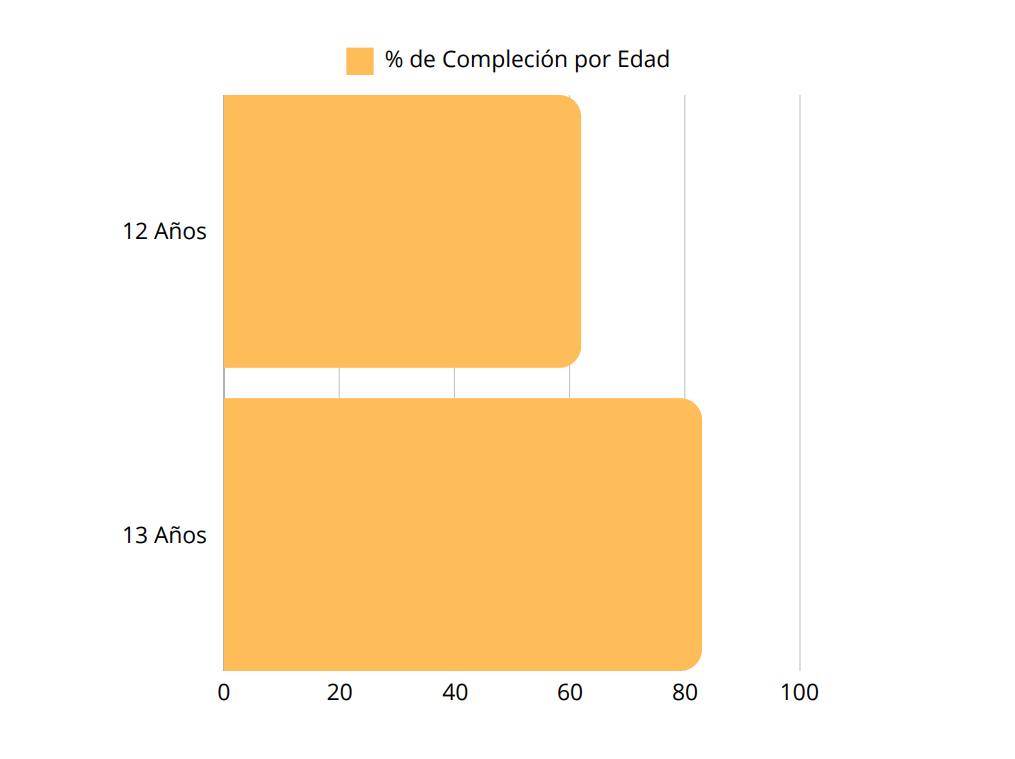
\includegraphics[width=350px,clip=true]{complecionporedad.png}
    \caption{Gráfica de complecion del prototipo por edad}
    \label{fig:paridad}
  \end{figure}

Además, en las Figuras \ref{fig:questionario_4}, \ref{fig:questionario_5}, \ref{fig:questionario_6} y \ref{fig:questionario_7} se puede observar cómo
 los alumnos sí que han entrenado su pensamiento computacional, donde el 67\% afirma haber practicado la depuración de errores, el 87\% comenta haber
  seguido un orden específico a la hora de seleccionar restauraciones que practicar (Lo que implica que estaban desarrollando algoritmia) y,
   finalmente, el 92\% de alumnos ha desarrollado el Análisis de Datos y la Generalización al leer los datos de las alteraciones y probolemas
   , y utilizar dicha información a la hora de restaurar problemas similares de distintos biomas.

Estas conclusiones se ven reflejadas en los datos recogidos en la Base de Datos, donde se puede ver claramente que pese a que el 40\% de todas las
 fases jugadas acabaron con un reinicio (Figura \ref{fig:fasesreiniciadas}), la mayoría de alumnos (Figura \ref{fig:fasescompletadas}) pudo completar el prototipo, 
 también se puede observar un alto grado de experimentación a la hora de jugar, dado que el 30\% de todas las máquinas colocadas a lo largo del experimento fueron vendidas (Figura \ref{fig:maquinasvendidas}). 

  \begin{figure}[H]
    \centering
      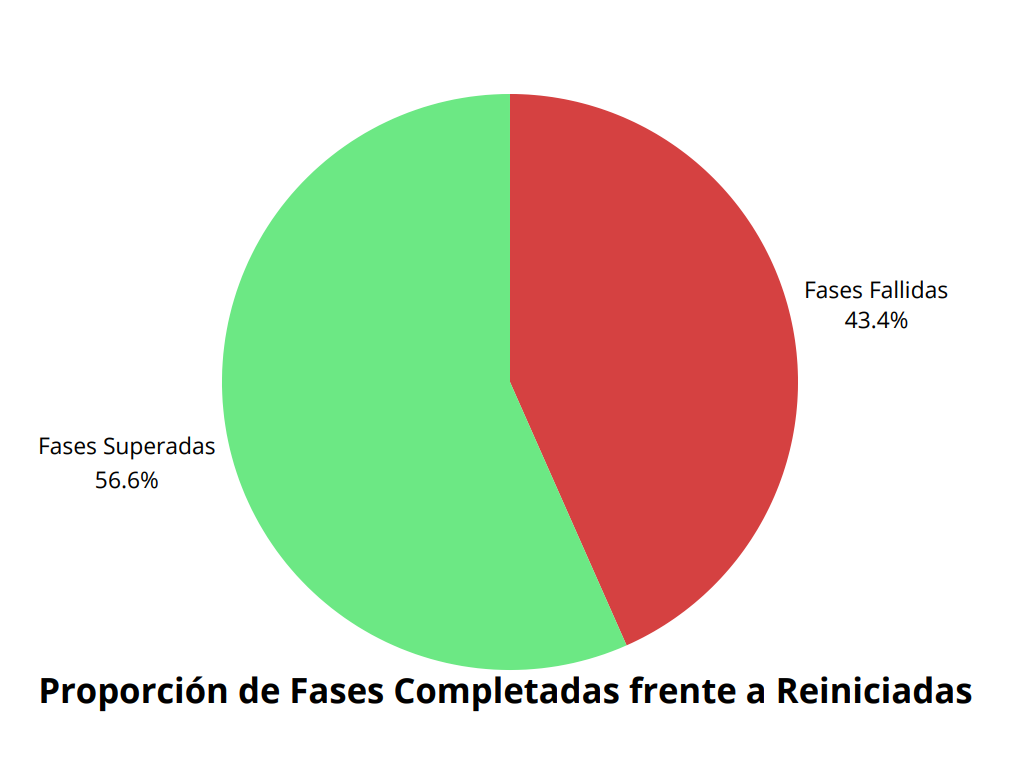
\includegraphics[width=350px,clip=true]{completadasfrentereiniciadas.png}
    \caption{Proporción de fases Completadas frente a Reiniciadas}
    \label{fig:fasesreiniciadas}
  \end{figure}

  \begin{figure}[H]
    \centering
      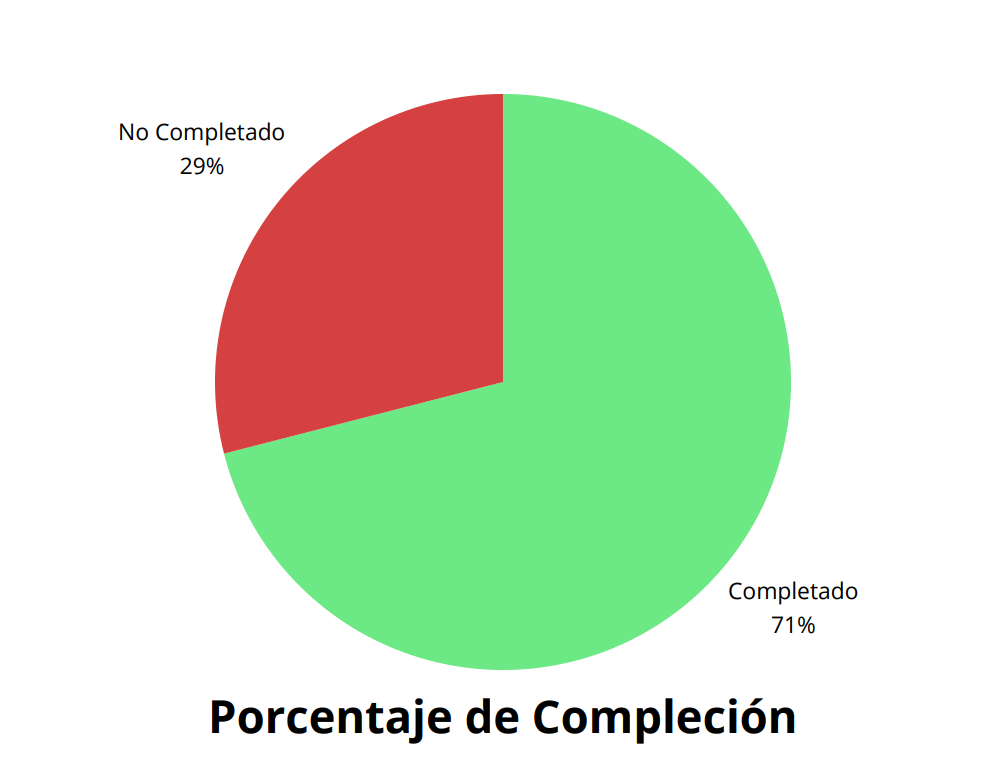
\includegraphics[width=350px,clip=true]{complecion.png}
    \caption{Proporción de partidas Completadas}
    \label{fig:fasescompletadas}
  \end{figure}

  \begin{figure}[H]
    \centering
      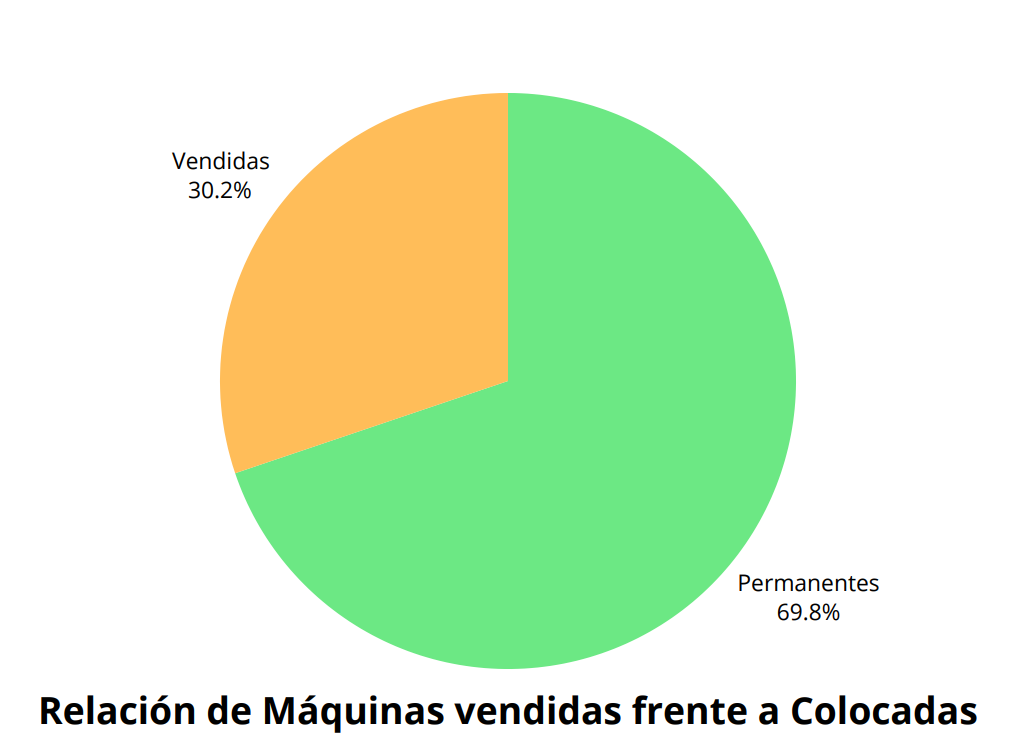
\includegraphics[width=350px,clip=true]{maquinasvendidas.png}
    \caption{Gráfica de total máquinas vendidas frente a colocadas}
    \label{fig:maquinasvendidas}
  \end{figure}
  
  Cabe destacar que pese a que pueda parecer que un 70\% de compleción podría no ser todo lo alto que pudiera esperarse, si se desglosa la progresión de los alumnos por la cantidad de fases que completaron (Figura \ref{fig:fasescompl}), 
  se puede observar que cerca del 92\% de los alumnos llegaron a completar más de la mitad de la demo, y que el 86\% pudo completar el 70\% del total de fases.

    \begin{figure}[H]
      \centering
        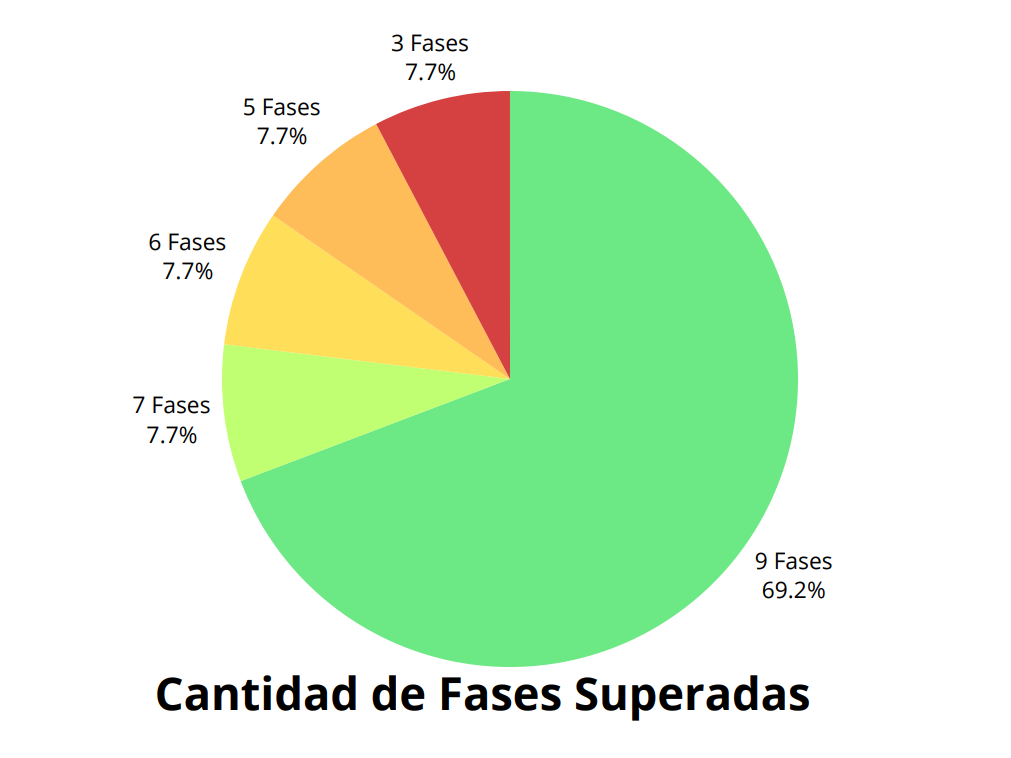
\includegraphics[width=350px,clip=true]{superadasporalumno.png}
      \caption{Cantidad de Fases Superadas por Alumno}
      \label{fig:fasescompl}
    \end{figure}

Es relevante quizás investigar dos ejemplos de alumnos que no fueron capaces de completar el juego, 'Pako' y 'Paula', por los resultados (Tabla \ref{fig:tablabbddpc}) podemos
 observar que 'Pako' se quedó atascado reintentando la misma fase una y otra vez, probablemente intentando colocar una máquina con 90\% de probabilidad
  de fallo, y 'Paula' no vendió ni una sola máquina, quizás provocando que se quedase sin dinero.

Otros datos a tener en cuenta son los de la Tabla \ref{fig:tablaResultadosPC}, donde se pueden encontrar testimonios en los que los alumnos indican 
sus partes favoritas del prototipo. En general queda patente que el sentimiento general hacia el juego es positivo, la opinión es que el juego es
 'divertido', 'original' y 'fácil de usar', pero además, merece la pena destacar que los propios alumnos opinan que ha sido una experiencia de 
 aprendizaje amena y divertida, 'mucho más divertida' al ser 'comparada con otros utensilios de clase'.